\chapter{Introduction}

%Replace \lipsum with text.
% You may have as many sections as you please. This is just for reference.

This thesis is a document to record our endeavour to tackle the problem of forming the social networks of Indian Politicians and Corporates and analysing them.

\section{Objective}
%\lipsum[1]

%You should cite papers in the following manner: Bayliss et al.~\cite{Bay1} gave an iterative method for Helmholtz equation etc.
%Similar work has been done in \cite{Bailey,Ernst,Gold3}.
The main idea is to collect data from semantic web (and other sources) to form a database ( here onwards we call it the \textbf{knowledge base} or \textbf{knowledge graph} )  and use it to for monitoring the top players in Indian society - mainly in the spheres of politics and businesses in India. We sought answers to questions like - 
\begin{itemize}
    \item \emph{Who were the big players in Indian politics and businesses?}
    \item \emph{Is there any influence (or possibility of it) of political field by a person in corporate field?}
    \item \emph{How important is one politician in a network of politicians (or a businessperson in a business network)?}
    \item \emph{On whom does actual power reside in a democracy?}
\end{itemize}

\section{Motivation \& Related Work}

In his book \textbf{The Power Elite} \cite{Mills}, C. Wright Mills calls attention to the interwoven interests of the leaders of the military, corporate, and political elements of society and suggests that the ordinary citizen is a relatively powerless subject of manipulation by those entities. His book deals with the power elite in US. But the hierarchy he proposes is more or less the same across all countries. Power rests with the top one percent in an economy. We plan to create a watchdog for that one percent. One interesting list to accompany this direction could be the Forbes list \cite{FORBES} of 147 companies that control everything. 

French economist Thomas Piketty in his famous work \textbf{Capital in the Twenty-First Century} \cite{Piketty} focuses on wealth and income inequality in Europe and the United States since the beginning of the industrial revolution. He proposes a global system of progressive wealth taxes to help reduce inequality and avoid the vast majority of wealth coming under the control of a tiny minority. We plan to collect, integrate, visualize and open such data for Indian terrain to let data fanatics carry out sych works to understand this inequality.

British writer and historian Patrick French, in his book \textbf{India: A Potrait} \cite{French} has stated many such interesting patterns in Indian politics where he argues that almost all of the young Indian politicians in the Indian Parliament are hereditary. Infact, patterns similar to this can be seen over the entire political Indian scene. One can find interesting overlaps, family ties, social links within these power houses. In a survey, \textbf{Who owns your media?} \cite{Media}, we find that even the media is an entity of importance and most of the politicians tend to try pull their strings in this domain. Another interesting case could be Jayant Sinha's family tree \cite{Sinha} and their business holdings. He is the Minister of State for Finance and a Member of Indian Parliament and has links to lot of powerful companies.

Research along the area have been prominent across countries. \textbf{Sastry} \cite{Sastry} shows how crime and money play important role in Indian elections. In a related work \textbf{Vaishnav} \cite{Essay} explain why do Indian parties elect criminal candidates and why they win. \textbf{Kapur} \cite{Builders} connects the hidden relationships between politicians and builders. He argues that where elections are costly but accountability mechanisms are weak, politicians often turn to private firms for illicit election finance and that where firms are highly regulated, politicians can exchange policy discretion or regulatory forbearance for bribes and monetary transfers from firms

Works like what we propose have already been done for countries like USA, UK, Chile etc. We have examples like \textbf{LittleSis} \cite{LilSis}, \textbf{Poderopedia} \cite{PODERO} where journalists, developers, analysts came together to put up profiles of important entities, institutions of the society and highlighted the connections between them. Littlesis (opposite of Big brother) in one hand exists in USA from the political and economical data available there. Poderopedia is a similar site in Chile. These sites feature separate pages of people in power in USA, their connections to different institutions and other entities , work history, visualizations of the connections to educate masses etc. Other than producing awareness to people about the corporate- political connections, these sites also allow public to register and collaborate in data entry processes and has an API system to promote further use of their data for research purposes.

Such system in absence of digital data/ structured data and other human factors is difficult in India. But various local and national initiatives have been started. \textbf{Association for democratic Reforms} \cite{ADR} for example has sites like \textbf{Myneta} \cite{MyNeta} to disseminate information about political leaders of India.	

Our vision is to produce a system similar in lines to the websites embedded with the power to query interesting connections, find interesting visualizations, and help raise suspicious issues.

\section{Merits}

The creation of such a system is beneficial for the society as a whole. It disemminates current information to public (or forms an indirect media for the same) which brings about accountability and transparency in the democracy. The project in the long run, helps to create a neat, structured minimal error data collection which otherwise is scattered at respective sources. Moreover, it also acts as a mashup data from different domains to be further used by journalists and academecians etc. Alongwith this, our work shows how such system of inter-disciplinary helps to find patterns and discover more informationa (with the challenges of building up a wiki based system to circulate information) .

\section{Detailed Goals}
In regard to above ideas, we splitted our goals to following objectives - 
\begin{enumerate}
    \item \textbf{Create a structured knowledgebase of corporate-political data.}
        Our main motive was to collect noisy semi structured data from various sources was the first problem encountered. This was followed by the task of entity resolution to merge repeated information pertaining to a single person. Finally the data was fitted into a model for easy queries.
    \item \textbf{Create a web portal to share and/or spread the information contained in the database.}
        The idea was to visualize the data contained in the knowledgebase. In lines with littlesis, we wanted to create a portal to show the networks obtained through different sources and add a wiki to add more through the crowd. Moreover, we also tried to give a minimal query engine to allow users to make custom queries for further analysis. We also wanted to create read/write apis to our knowledge database to help app writers to easily extend it to their applications.
    \item \textbf{Analysis to find patterns in data.}
        Our endeavour is to use the knowledge graph and the query engine we tried to build to look into the network properties and find new patterns and information out of it.

\end{enumerate}
% You may add figures in the following manner.
%\begin{figure}[here]
%\begin{center}	
%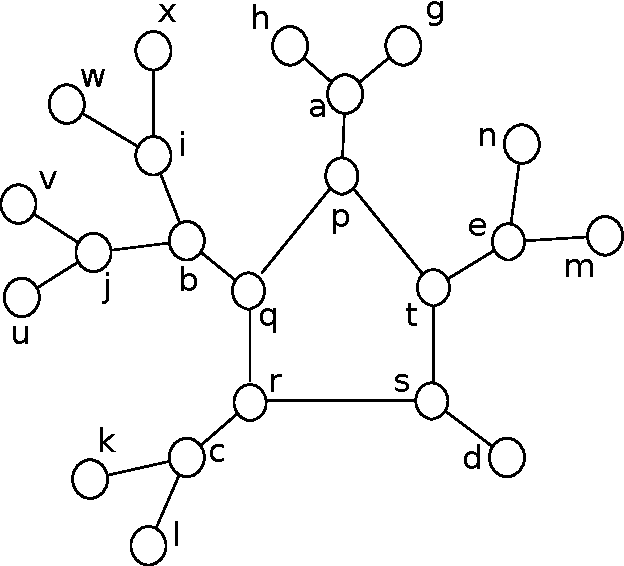
\includegraphics[scale=0.4]{pent} 
%\caption{Pentagon $pqrst$}
%\label{fig:pent}
%\end{center}
%\end{figure}

%\lipsum[1]

%\section{SECTION NAME}
%\lipsum[2]

%\begin{table}
%\centering
%\begin{tabular}{| c | c |}
%\hline
%{\bf item 1} & {\bf item 2} \\ \hline
%
%abcde & 5 \\ \hline
%
%pqrst & 4 \\ \hline
%\end{tabular}
%\caption{A sample table}
%\label{table:1}
%\end{table}
